\title{\textbf{FlashAttention-3 FP8: Low-Precision 8-bit Attention with Hardware-Aware Fallback}

\author{Anonymous authors}



\section{Introduction}

\subsection{Motivation}

The memory cost of attention has been a bottleneck for transformer inference 
since Vaswani et al. (2017). The intermediate attention matrix $Q K\^{}\top \in 
\mathbb{R}\^{}{L \times L}$ requires $\mathcal{O}(L\^{}2)$ memory, which for 
$L = 8192$ and 16-bit precision is 128 MB per head -- infeasible for 
long-context applications.

FlashAttention (Dao et al., 2022) solved this by \textbf{tiling} the attention 
computation in GPU SRAM, achieving exact attention with $\mathcal{O}(L)$ 
memory. FlashAttention-2 (Dao, 2023) improved parallelism across the sequence 
dimension and reduced non-matmul FLOPs. FlashAttention-3 (Shah et al., 2024) 
added \textbf{asynchronous hardware overlap} on Hopper GPUs and, crucially, 
\textbf{FP8 tensor core support}, which roughly doubles throughput on H100-class 
hardware.

0.85


\subsection{Problem Statement}

We seek an attention implementation $\mathcal{A}$ such that:

\begin{enumerate}
\item \textbf{Exact or near-exact}: $\mathcal{A}(Q, K, V) \approx \text{softmax}(QK^\top/\sqrt{d})V$
\item \textbf{Memory-efficient}: $\mathcal{O}(L)$ peak memory, not $\mathcal{O}(L^2)$
\item \textbf{Hardware-portable}: works on any CUDA GPU, using FP8 when available
\item \textbf{Weight-compatible}: preserves pretrained weights without retraining
\item \textbf{Fine-tunable}: supports LoRA recovery when needed

\end{enumerate}
\subsection{Our Approach}

We implement FlashAttention-3 with three design principles:

\begin{enumerate}
\item \textbf{Runtime hardware detection.} At construction time, we check for
  \texttt{torch.float8\_e4m3fn} support and the presence of \texttt{flash\_attn} /
  \texttt{flash\_attn\_interface}. The FP8 path is used only if both are available.

\item \textbf{Correct fallback to SDPA.} If the FP8 path is unavailable, we use
  PyTorch's built-in \texttt{F.scaled\_dot\_product\_attention}, which internally
  dispatches to FlashAttention-2 or memory-efficient attention depending on
  the CUDA version.

\item \textbf{Exact weight transfer.} Base weights are copied from the pretrained
  attention with architecture-specific handling for Conv1D (GPT-2), nested
  self-attention (RoBERTa), and GQA (Qwen).

\end{enumerate}
\subsection{Contributions}

\begin{itemize}
\item \textbf{A hardware-aware FP8 attention implementation} that runs correctly
  across four transformer families and gracefully degrades on non-Hopper
  hardware.
\item \textbf{An honest evaluation} reporting that on our test hardware (RTX 4070
  Laptop), FP8 tensor cores are not exposed, so the FP8 path is never
  taken. We identify the exact hardware needed to reproduce the FP8
  speedups.
\item \textbf{An accuracy-preservation study} showing that when the fallback path is
  used, accuracy matches the baseline within \textbf{-0.92\%} on DistilBERT,
  \textbf{0.85\%} on RoBERTa, and \textbf{0.85\%} on GPT-2.
\item \textbf{Full reproducibility}, including hardware-detection logic and LoRA
  configuration.

\end{itemize}
\subsection{Paper Organization}

Section 2 reviews related work on FlashAttention and FP8 training. Section 3 
provides background on attention, FP8 formats, and LoRA. Section 4 presents 
our implementation. Section 5 describes architecture integration. Section 6 
details the experimental setup. Section 7 reports results. Section 8 
analyzes why FP8 is unavailable on our hardware. Section 9 discusses 
practical guidance. Section 10 lists limitations. Section 11 concludes.



\subsection{Notation}

\begin{table}[H]
\centering
\small
\begin{tabular}{lll}
\toprule
\textbf{Symbol} & \textbf{Meaning} & \textbf{First appears} \\
\midrule
$L$ & Sequence length & 3.1 \\
$d$ & Head dimension & 3.1 \\
$H$ & Number of query heads & 3.1 \\
$H_{kv}$ & Number of KV heads & 3.2 \\
$B$ & Batch size & 3.1 \\
$S$ & SRAM tile size (FlashAttention) & 3.3 \\
$r$ & LoRA rank & 3.5 \\
$\text{fp8}$ & 8-bit float format (e4m3fn or e5m2) & 3.4 \\
\bottomrule
\end{tabular}
\end{table}
</parameter>




\section{Related Work}

\subsection{Efficient Exact Attention}

\subsubsection{FlashAttention Series}

\textbf{FlashAttention} (Dao et al., 2022). Introduces tiling to keep the 
$L \times L$ attention matrix in SRAM. Memory drops from $\mathcal{O}(L^2)$ 
to $\mathcal{O}(L)$; recomputation in the backward pass avoids storing 
intermediate activations.

\textbf{FlashAttention-2} (Dao, 2023). Improves parallelism over the sequence 
dimension, reduces non-matmul FLOPs (rescaling, masking), and enables 
sequence-parallel training.

\textbf{FlashAttention-3} (Shah et al., 2024). Adds Hopper-specific features:
\begin{itemize}
\item \textbf{TMA (Tensor Memory Accelerator)} for asynchronous loads
\item \textbf{Warpgroup specialization} (producer/consumer)
\item \textbf{FP8 support} (e4m3 for Q/K, e5m2 for V or vice versa)
\item \textbf{Pipelined softmax} overlapping with matrix multiplication

\end{itemize}
\subsubsection{Memory-Efficient Attention}

PyTorch's \texttt{F.scaled\_dot\_product\_attention} (SDPA) dispatches to one of 
several backends: FlashAttention-2, memory-efficient attention (xFormers), 
or the native CUDA path. We use SDPA as the fallback.

\subsubsection{Other Exact Attention}

\textbf{Memory-efficient attention} (Rabe \& Staats, 2021). Reduces memory by 
recomputing activations during backward.

\textbf{PagedAttention} (Kwon et al., 2023). Manages KV cache in pages for 
serving.

\subsection{Low-Precision Attention}

\subsubsection{FP8 Training}

\textbf{FP8 for Deep Learning} (Micikevicius et al., 2022). Defines the e4m3 and 
e5m2 formats and provides recipes for stable training.

\textbf{TransformerEngine} (NVIDIA, 2023). A library that automatically casts 
activations to FP8 during training.

\textbf{FP8-LM} (Peng et al., 2023). Shows that FP8 training matches BF16 
accuracy for large language models.

\subsubsection{Quantization}

\textbf{LLM.int8()} (Dettmers et al., 2022). 8-bit inference with outlier handling.

\textbf{GPTQ} (Frantar et al., 2023). Post-training quantization using second-order 
information.

\textbf{AWQ} (Lin et al., 2023). Activation-aware weight quantization.

\subsection{Position of Our Work}

Our implementation differs from prior work in three ways:

\begin{table}[H]
\centering
\small
\begin{tabular}{lll}
\toprule
\textbf{Axis} & \textbf{Prior work} & \textbf{Ours} \\
\midrule
\textbf{Hardware assumption} & Assumes specific architecture & Detects at runtime \\
\textbf{Fallback path} & Error or requires reinstall & SDPA \\
\textbf{Architecture support} & Usually one family & Four families \\
\textbf{Weight transfer} & Not addressed & Exact copy \\
\bottomrule
\end{tabular}
\end{table}

\textbf{Key distinction.} The original FlashAttention-3 paper (Shah et al., 2024) 
reports speedups on H100. Our contribution is \textbf{portability} -- a version 
that runs correctly on any GPU, using FP8 when available. We do not claim 
to match the H100 speedups on non-Hopper hardware.



\subsection{Comparison Table}

\begin{table}[H]
\centering
\small
\begin{tabular}{lllllll}
\toprule
\textbf{Implementation} & \textbf{FP8?} & \textbf{Fallback?} & \textbf{DistilBERT?} & \textbf{RoBERTa?} & \textbf{GPT-2?} & \textbf{Qwen?} \\
\midrule
FlashAttention-2 & No & Error & Manual & Manual & Manual & Manual \\
FlashAttention-3 & Yes & Error & Manual & Manual & Manual & Manual \\
PyTorch SDPA & No & -- & Manual & Manual & Manual & Manual \\
\textbf{Ours} & \textbf{Yes} & \textbf{SDPA} & \textbf{Yes} & \textbf{Yes} & \textbf{Yes} & \textbf{Yes} \\
\bottomrule
\end{tabular}
\end{table}




\section{Background}

\subsection{Scaled Dot-Product Attention}

Standard attention:

\[
\text{Attn}(Q, K, V) = \text{softmax}\!\left(\frac{Q K^\top}{\sqrt{d}}\right) V
\tag{3.1}
\]

Memory for $QK^\top$ is $\mathcal{O}(BL^2)$ -- the target of reduction.

\subsection{Grouped-Query Attention (GQA)}

GQA uses $H_{kv} < H$ to reduce KV-cache size:

\[
K, V \in \mathbb{R}^{B \times L \times H_{kv} d}, \qquad
H_{\text{repeat}} = H / H_{kv}
\tag{3.2}
\]

The \texttt{repeat\_kv} operation expands KV to match Q heads.

\subsection{FlashAttention Tiling}

FlashAttention partitions $Q, K, V$ into blocks that fit in SRAM ($\sim$ 100 KB 
on A100, $\sim$ 200 KB on H100). The inner loop:

\[
O_{ij} \leftarrow \text{softmax}(Q_i K_j^\top / \sqrt{d}) V_j
\tag{3.3}
\]

accumulates partial results in SRAM, never materializing $QK^\top$ to HBM.

\textbf{Tiling cost.} For block size $S$, the number of HBM reads is 
$\mathcal{O}(BL \cdot S)$, and SRAM occupancy is $\mathcal{O}(S^2 + Sd)$.

\subsection{FP8 Format}

The 8-bit floating-point format has two variants (Micikevicius et al., 2022):

\begin{table}[H]
\centering
\small
\begin{tabular}{llll}
\toprule
\textbf{Format} & \textbf{Bits (sign/exp/mant)} & \textbf{Max} & \textbf{Precision} \\
\midrule
E4M3 & 1 / 4 / 3 & 448 & ~0.5\% \\
E5M2 & 1 / 5 / 2 & 57344 & ~1\% \\
\bottomrule
\end{tabular}
\end{table}

\textbf{FP8 tensor cores.} Only Hopper (H100, H200) and Ada (RTX 4090, L40) expose 
FP8 tensor cores with 2$$\times$ throughput over FP16. On Ampere (A100, RTX 30-series) 
and earlier, FP8 is only a storage format, not a compute format.

\textbf{Detection.} PyTorch exposes the FP8 dtype as \texttt{torch.float8\_e4m3fn} 
(available in PyTorch $\ge$ 2.1). Its presence in \texttt{dir(torch)} indicates the 
build supports the type, but \textbf{does not} indicate hardware tensor-core 
support. This must be verified at runtime via CUDA capability.

\subsection{LoRA}

LoRA (Hu et al., 2021) parameterizes:

\[
\Delta W = \frac{\alpha}{r} BA, \quad
A \in \mathbb{R}^{r \times k}, \quad
B \in \mathbb{R}^{d \times r}
\tag{3.4}
\]

with $B = 0$ at init. Only $A, B$ are trained.

\subsection{Hardware Capabilities}

\begin{table}[H]
\centering
\small
\begin{tabular}{llll}
\toprule
\textbf{GPU} & \textbf{Architecture} & \textbf{Compute Capability} & \textbf{FP8 Tensor Cores?} \\
\midrule
A100 & Ampere & 8.0 &  \\
H100 & Hopper & 9.0 &  \\
H200 & Hopper & 9.0 &  \\
RTX 3090 & Ampere & 8.6 &  \\
RTX 4070 & Ada & 8.9 & (driver-dependent) \\
RTX 4090 & Ada & 8.9 &  \\
\bottomrule
\end{tabular}
\end{table}

On RTX 4070 Laptop (this study's hardware), FP8 tensor cores exist 
architecturally but are often not exposed through the CUDA driver; we 
detect this and fall back.

\subsection{Notation Summary}

\begin{table}[H]
\centering
\small
\begin{tabular}{ll}
\toprule
\textbf{Symbol} & \textbf{Meaning} \\
\midrule
$B$ & Batch size \\
$L$ & Sequence length \\
$d$ & Head dimension \\
$H$ & Query head count \\
$H_{kv}$ & KV head count \\
$r$ & LoRA rank \\
$S$ & SRAM block size \\
$f_{p8}$ & FP8 format (e4m3 or e5m2) \\
\bottomrule
\end{tabular}
\end{table}




\section{Method}

\subsection{Overview}

Our implementation wraps FlashAttention-3 with three layers of safety:

\begin{enumerate}
\item \textbf{Import-time detection.} At module load, we attempt to import
  \texttt{flash\_attn\_interface} or \texttt{flash\_attn}. If neither is available, we set
  \texttt{FLASH\_ATTN\_AVAILABLE = False}.

\item \textbf{Runtime FP8 detection.} At each forward, we check that:
\end{enumerate}
\begin{itemize}
\item \texttt{FLASH\_ATTN\_AVAILABLE} is True
\item \texttt{self.use\_fp8} is True
\item \texttt{q.is\_cuda} is True
\item \texttt{torch.float8\_e4m3fn} is available
  
  If all hold, we cast Q/K/V to FP8 and call \texttt{flash\_attn\_func}.

\end{itemize}
\begin{enumerate}
\item \textbf{SDPA fallback.} If any check fails, we call
  \texttt{F.scaled\_dot\_product\_attention} instead.

\end{enumerate}
\begin{lstlisting}
              +-----------------------------+
              |  Input Q, K, V              |
              +--------------+--------------+
                             |
                              
              +-----------------------------+
              |  FLASH_ATTN_AVAILABLE ?     |
              +------+--------------+-------+
                     | No           | Yes
                     |              |
                     |               
                     |    +-----------------+
                     |    | self.use_fp8 ?  |
                     |    +--+---------+----+
                     |       | No      | Yes
                     |       |         |
                     |       |          
                     |       |   +--------------+
                     |       |   | has float8? |
                     |       |   +--+-------+---+
                     |       |      | No    | Yes
                     |       |      |       |
                     |                       
                     |    +----------------------+
                     +--- |  SDPA fallback       |
                          +----------------------+
                                    |
                                     
                          +----------------------+
                          |  Output              |
                          +----------------------+
\end{lstlisting}

\subsection{Detection Logic}

\subsubsection{FlashAttention Import}

\begin{lstlisting}
try:
    from flash_attn_interface import flash_attn_func
    FLASH_ATTN_AVAILABLE = True
except ImportError:
    try:
        from flash_attn import flash_attn_func
        FLASH_ATTN_AVAILABLE = True
    except ImportError:
        FLASH_ATTN_AVAILABLE = False
\end{lstlisting}

The first import path is used by the Hopper-optimized \texttt{flash-attn-3} package; 
the second by the community \texttt{flash-attn} package.

\subsubsection{FP8 Path Condition}

At each forward, we check four conditions:

\begin{lstlisting}
use_fp8_path = (
    FLASH_ATTN_AVAILABLE
    and self.use_fp8
    and q.is_cuda
    and hasattr(torch, "float8_e4m3fn")
)
\end{lstlisting}

\textbf{Note.} We do \textbf{not} check CUDA capability directly; if the hardware 
does not support FP8, \texttt{flash\_attn\_func} will raise a runtime error and we 
catch it, falling back to SDPA.

\subsection{FP8 Cast}

When the FP8 path is taken:

\begin{lstlisting}
q_fa = q.transpose(1, 2).contiguous().to(torch.float8_e4m3fn)
k_fa = k.transpose(1, 2).contiguous().to(torch.float8_e4m3fn)
v_fa = v.transpose(1, 2).contiguous().to(torch.float8_e4m3fn)
out = flash_attn_func(q_fa, k_fa, v_fa, causal=causal_flag).to(dtype)
\end{lstlisting}

\textbf{Cast order.} Q and K are cast to e4m3 (higher precision for products); 
V is cast to the same. The output is returned in FP16/BF16.

\textbf{No scaling.} Unlike TransformerEngine, we do not apply per-tensor scaling. 
This is correct for well-behaved distributions but may lose precision for 
models with large activations.

\subsection{SDPA Fallback}

If the FP8 path is not taken:

\begin{lstlisting}
if causal_flag and attn_mask is None:
    out_sdpa = F.scaled_dot_product_attention(
        q, k, v, attn_mask=None, is_causal=True, dropout_p=self.dropout.p
    )
else:
    # Build causal mask, add padding mask
    out_sdpa = F.scaled_dot_product_attention(
        q, k, v, attn_mask=attn_mask, is_causal=False, dropout_p=self.dropout.p
    )
\end{lstlisting}

PyTorch's SDPA dispatches internally to:
\begin{itemize}
\item FlashAttention-2 (if installed and CUDA >= 11.8)
\item Memory-efficient attention
\item Native math

\end{itemize}
\subsection{Architecture-Specific Weight Transfer}

The \texttt{copy\_weights} method extracts Q, K, V, and output projections from four 
families:

\subsubsection{GPT-2 (Fused Conv1D)}

\begin{lstlisting}
if hasattr(src, "c_attn"):
    w = src.c_attn.weight.data
    if src.c_attn.__class__.__name__ == "Conv1D":
        w = w.t()  # (in, out) $\to$ (out, in)
    q_w, k_w, v_w = w.chunk(3, dim=0)
    extracted["q"] = (q_w, ...)
    ...
\end{lstlisting}

\subsubsection{RoBERTa (Nested)}

\begin{lstlisting}
elif hasattr(src, "self") and hasattr(src.self, "query"):
    q_w = src.self.query.weight.data
    k_w = src.self.key.weight.data
    v_w = src.self.value.weight.data
    if hasattr(src.output, "dense"):
        o_w = src.output.dense.weight.data
\end{lstlisting}

\subsubsection{DistilBERT (Flat)}

\begin{lstlisting}
else:
    q_w = src.q_lin.weight.data
    k_w = src.k_lin.weight.data
    v_w = src.v_lin.weight.data
    o_w = src.out_lin.weight.data
\end{lstlisting}

\subsubsection{Qwen (GQA + RoPE)}

Qwen uses separate \texttt{q\_proj}, \texttt{k\_proj}, \texttt{v\_proj}, \texttt{o\_proj}. Standard extraction.

\subsection{Nested Encoder Bypass}

For RoBERTa and other BERT-family models, the output projection lives 
outside the self-attention module:

\begin{lstlisting}
BertAttention
+-- self: BertSelfAttention
|   +-- query
|   +-- key
|   +-- value
+-- output: BertSelfOutput
    +-- dense  $\leftarrow$ output projection
\end{lstlisting}

We set \texttt{is\_nested\_encoder = True}, which causes \texttt{forward} to return raw 
\texttt{context} (without applying \texttt{out\_proj}). The outer \texttt{output.dense} applies 
the projection.

For DistilBERT, \texttt{out\_lin} is inside the attention module, so we set 
\texttt{is\_nested\_encoder = False}.

\subsection{LoRA Adaptation}

Each projection is wrapped in \texttt{LoRALinear}:

\begin{lstlisting}
class LoRALinear(nn.Module):
    def __init__(self, in_features, out_features, ..., lora_rank=16):
        self.weight = nn.Parameter(...)      # frozen after copy
        self.lora_A = nn.Parameter(...)      # trainable
        self.lora_B = nn.Parameter(...)      # trainable, initialized to 0
    
    def forward(self, x):
        out = F.linear(x, self.weight, self.bias)
        if self.lora_rank > 0:
            out += F.linear(F.linear(x, self.lora_A), self.lora_B) * self.lora_scaling
        return out
\end{lstlisting}

\subsection{Complexity Analysis}

\begin{table}[H]
\centering
\small
\begin{tabular}{lll}
\toprule
\textbf{Component} & \textbf{Time} & \textbf{Memory} \\
\midrule
Q/K/V projection & $\mathcal{O}(BLd^2)$ & $\mathcal{O}(BLd)$ \\
FlashAttention-3 FP8 & $\mathcal{O}(BL^2 d / S)$ & $\mathcal{O}(BLd + S^2)$ \\
SDPA (fallback) & $\mathcal{O}(BL^2 d)$ & $\mathcal{O}(BLd)$ \\
Output projection & $\mathcal{O}(BLd^2)$ & $\mathcal{O}(BLd)$ \\
\bottomrule
\end{tabular}
\end{table}

\textbf{FP8 path} uses ~$S^2$ SRAM per tile and reads Q/K/V once from HBM.

\textbf{SDPA path} uses memory-efficient attention with the same asymptotics but 
without the FP8 speedup.

\subsection{Parameter Analysis}

Our implementation \textbf{does not reduce parameter count}. The LoRA adapters 
add:

\[
\Delta p = r \cdot (d_\text{in} + d_\text{out})
\tag{4.1}
\]

per layer. For $r = 16$ and $d = 768$, this is 24,576 params per projection.

\textbf{Total overhead (DistilBERT):} 4 projections $$\times$ 6 layers $$\times$ 24,576 = 
\textbf{589,824 params} (+0.88\%).

\textbf{This is not a compression method.}

\subsection{Algorithm}

\textbf{Algorithm 1:} FlashAttention3FP8 forward pass
\begin{lstlisting}
Input:  X $\in$ R^{B$$\times$L$$\times$d}, attention_mask
Output: Y $\in$ R^{B$$\times$L$$\times$d}

 1: Q $\leftarrow$ X W_Q;  K $\leftarrow$ X W_K;  V $\leftarrow$ X W_V      With LoRA
 2: if RoPE: (Q, K) $\leftarrow$ Rotary(Q, K)
 3: if GQA:  (K, V) $\leftarrow$ repeat_kv(K, V)
 4:
 5: if FLASH_ATTN_AVAILABLE AND use_fp8 AND q.is_cuda AND has_float8:
 6:     q8, k8, v8 $\leftarrow$ cast_to_fp8(Q, K, V)
 7:     try:
 8:         out $\leftarrow$ flash_attn_func(q8, k8, v8, causal)
 9:     except:
10:         out $\leftarrow$ NULL    Fallback
11: else:
12:     out $\leftarrow$ NULL
13:
14: if out is NULL:
15:     out $\leftarrow$ SDPA(Q, K, V, mask, causal)
16:
17: if not is_nested_encoder:
18:     out $\leftarrow$ out_proj(out)
19: return out
\end{lstlisting}




\section{Architecture Integration}

\subsection{Model Support Matrix}

\begin{table}[H]
\centering
\small
\begin{tabular}{llllll}
\toprule
\textbf{Architecture} & \textbf{Class} & \textbf{Nested?} & \textbf{RoPE?} & \textbf{GQA?} & \textbf{FP8 on RTX 4070?} \\
\midrule
DistilBERT & \texttt{MultiHeadSelfAttention} & No & No & No & Fallback \\
RoBERTa & \texttt{BertSelfAttention} & Yes & No & No & Fallback \\
GPT-2 & \texttt{GPT2Attention} (Conv1D) & No & No & No & Fallback \\
Qwen3.5 & \texttt{Qwen3Attention} & No & Yes & Yes & Fallback \\
\bottomrule
\end{tabular}
\end{table}

\subsection{Weight Transfer Details}

\subsubsection{Conv1D Orientation (GPT-2)}

HuggingFace \texttt{Conv1D} stores weight as \texttt{(in\_features, out\_features)}:

\begin{lstlisting}
class Conv1D(nn.Module):
    def __init__(self, nf, nx):
        self.weight = nn.Parameter(torch.empty(nx, nf))
        # nx = in_features, nf = out_features
\end{lstlisting}

Our extraction:

\begin{lstlisting}
if src.c_attn.__class__.__name__ == "Conv1D":
    w = src.c_attn.weight.data.t()  # $\to$ (nf, nx)
\end{lstlisting}

We detect Conv1D via class name \textbf{or} the shape heuristic 
\texttt{w.shape[0] < w.shape[1]} (which holds for Conv1D with $n_f > n_x$ but 
not for square matrices).

\subsubsection{Nested vs Flat Detection}

We use the following logic in \texttt{copy\_weights}:

\begin{lstlisting}
if hasattr(src, "out_lin"):
    is_nested = False       # DistilBERT
elif (hasattr(src, "self") and hasattr(src.self, "query")
      and hasattr(src, "output") and hasattr(src.output, "dense")):
    is_nested = True        # RoBERTa
elif cls_name in ["BertSelfAttention", "RobertaSelfAttention", ...]:
    is_nested = True
elif cls_name.endswith("SelfAttention") and "distil" not in cls_name.lower():
    is_nested = True
else:
    is_nested = False
\end{lstlisting}

\textbf{Key insight:} check \texttt{out\_lin} \textbf{first}. DistilBERT's 
\texttt{MultiHeadSelfAttention} ends with "SelfAttention" and would be misclassified 
as nested otherwise.

\subsection{GQA Support}

For Qwen3.5 with $H_{kv} = 2 < H = 8$:

\begin{lstlisting}
# In forward:
if self.num_kv_heads != self.num_heads:
    k = repeat_kv(k, self.kv_repeat)
    v = repeat_kv(v, self.kv_repeat)
\end{lstlisting}

The \texttt{repeat\_kv} function expands via broadcast and reshape:

\begin{lstlisting}
def repeat_kv(hidden_states, n_rep):
    if n_rep == 1:
        return hidden_states
    B, H_kv, L, D = hidden_states.shape
    hidden_states = hidden_states[:, :, None, :, :].expand(B, H_kv, n_rep, L, D)
    return hidden_states.reshape(B, H_kv * n_rep, L, D)
\end{lstlisting}

\subsection{RoPE Support}

We support partial RoPE, where the rotary dimension is smaller than 
\texttt{head\_dim}:

\begin{lstlisting}
def apply_rotary_pos_emb(q, k, cos, sin):
    rotary_dim = cos.shape[-1]
    if rotary_dim < q.shape[-1]:
        q_rot, q_pass = q[..., :rotary_dim], q[..., rotary_dim:]
        q_rot_embed = q_rot * cos + rotate_half(q_rot) * sin
        q = torch.cat([q_rot_embed, q_pass], dim=-1)
    ...
\end{lstlisting}

\subsection{Causality}

For decoder models, we set \texttt{causal\_flag = True} if:
\begin{itemize}
\item \texttt{self.is\_decoder}
\item AND not cross-attention
\item AND $L = L_{kv}$

\end{itemize}
This ensures we only apply causal masking for self-attention, not 
cross-attention.

\subsection{Injection Algorithm}

\textbf{Algorithm 2:} Inject FlashAttention3FP8 into a layer
\begin{lstlisting}
Input:  layer   (transformer block), config, old_attn
Output: new attention module in  

1: new $\leftarrow$ FlashAttention3FP8(config, old_attn=old_attn)
2: if new.copy_weights failed: return None
3: if   has .attention.self:
4:      .attention.self $\leftarrow$ new
5:     new.is_nested_encoder $\leftarrow$ True
6: elif   has .attention:
7:      .attention $\leftarrow$ new
8: elif   has .self_attn:
9:      .self_attn $\leftarrow$ new
10: return new
\end{lstlisting}

\subsection{Failure Handling}

\begin{table}[H]
\centering
\small
\begin{tabular}{lll}
\toprule
\textbf{Failure} & \textbf{Detection} & \textbf{Response} \\
\midrule
\texttt{flash\_attn} not installed & ImportError & \texttt{FLASH\_ATTN\_AVAILABLE = False} \\
\texttt{float8\_e4m3fn} missing & \texttt{hasattr(torch, ...)} & Skip FP8 path \\
FP8 kernel crash & try/except & SDPA fallback \\
Weight copy failure & Frobenius check & Log + skip \\
Cross-attention & \texttt{encoder\_hidden\_states != None} & Not supported -- raise \\
\bottomrule
\end{tabular}
\end{table}

\subsection{Cross-Attention}

Our implementation \textbf{does not support cross-attention} in the current 
version. If \texttt{encoder\_hidden\_states} is provided, we raise 
\texttt{NotImplementedError}. This is acceptable because the models tested 
(DistilBERT, RoBERTa, GPT-2) are encoder-only or decoder-only.

\subsection{Common Pitfalls}

\subsubsection{Nested Encoder Double-Projection}

If \texttt{is\_nested\_encoder} is set incorrectly, the output projection is applied 
twice (once inside our module, once by the outer block):

\begin{lstlisting}
# WRONG for RoBERTa
if not self.is_nested_encoder:
    out = self.out_proj(out)  # would double-project
\end{lstlisting}

We verify \texttt{is\_nested\_encoder} by checking \texttt{hasattr(src, "out\_lin")}.

\subsubsection{Conv1D Transpose}

If we forget to transpose Conv1D weights, Q/K/V shapes mismatch:

\begin{lstlisting}
# CORRECT
w = src.c_attn.weight.data.t()
\end{lstlisting}

\subsubsection{GQA Mismatch}

If \texttt{num\_kv\_heads} is wrong, \texttt{view(B, L, num\_kv\_heads, head\_dim)} will fail 
or silently produce wrong results. We detect the correct value from 
\texttt{config.num\_key\_value\_heads}.

\subsection{Registry}

\begin{lstlisting}
@ATTENTION_REGISTRY.register("flash3_fp8")
@ATTENTION_REGISTRY.register("flash_attention3_fp8")
class FlashAttention3FP8(BaseAttention):
    ...
\end{lstlisting}

\subsection{Integration with LoRA Recovery}

The pipeline:

\begin{enumerate}
\item Load base model.
\item Replace attention with \texttt{FlashAttention3FP8} via injection.
\item Freeze base weights, keep LoRA trainable.
\item Run recovery fine-tuning for 50 steps.
\item Evaluate.

\end{enumerate}
This is the same pipeline as other modules in our framework.



\begin{figure}[H]
\centering
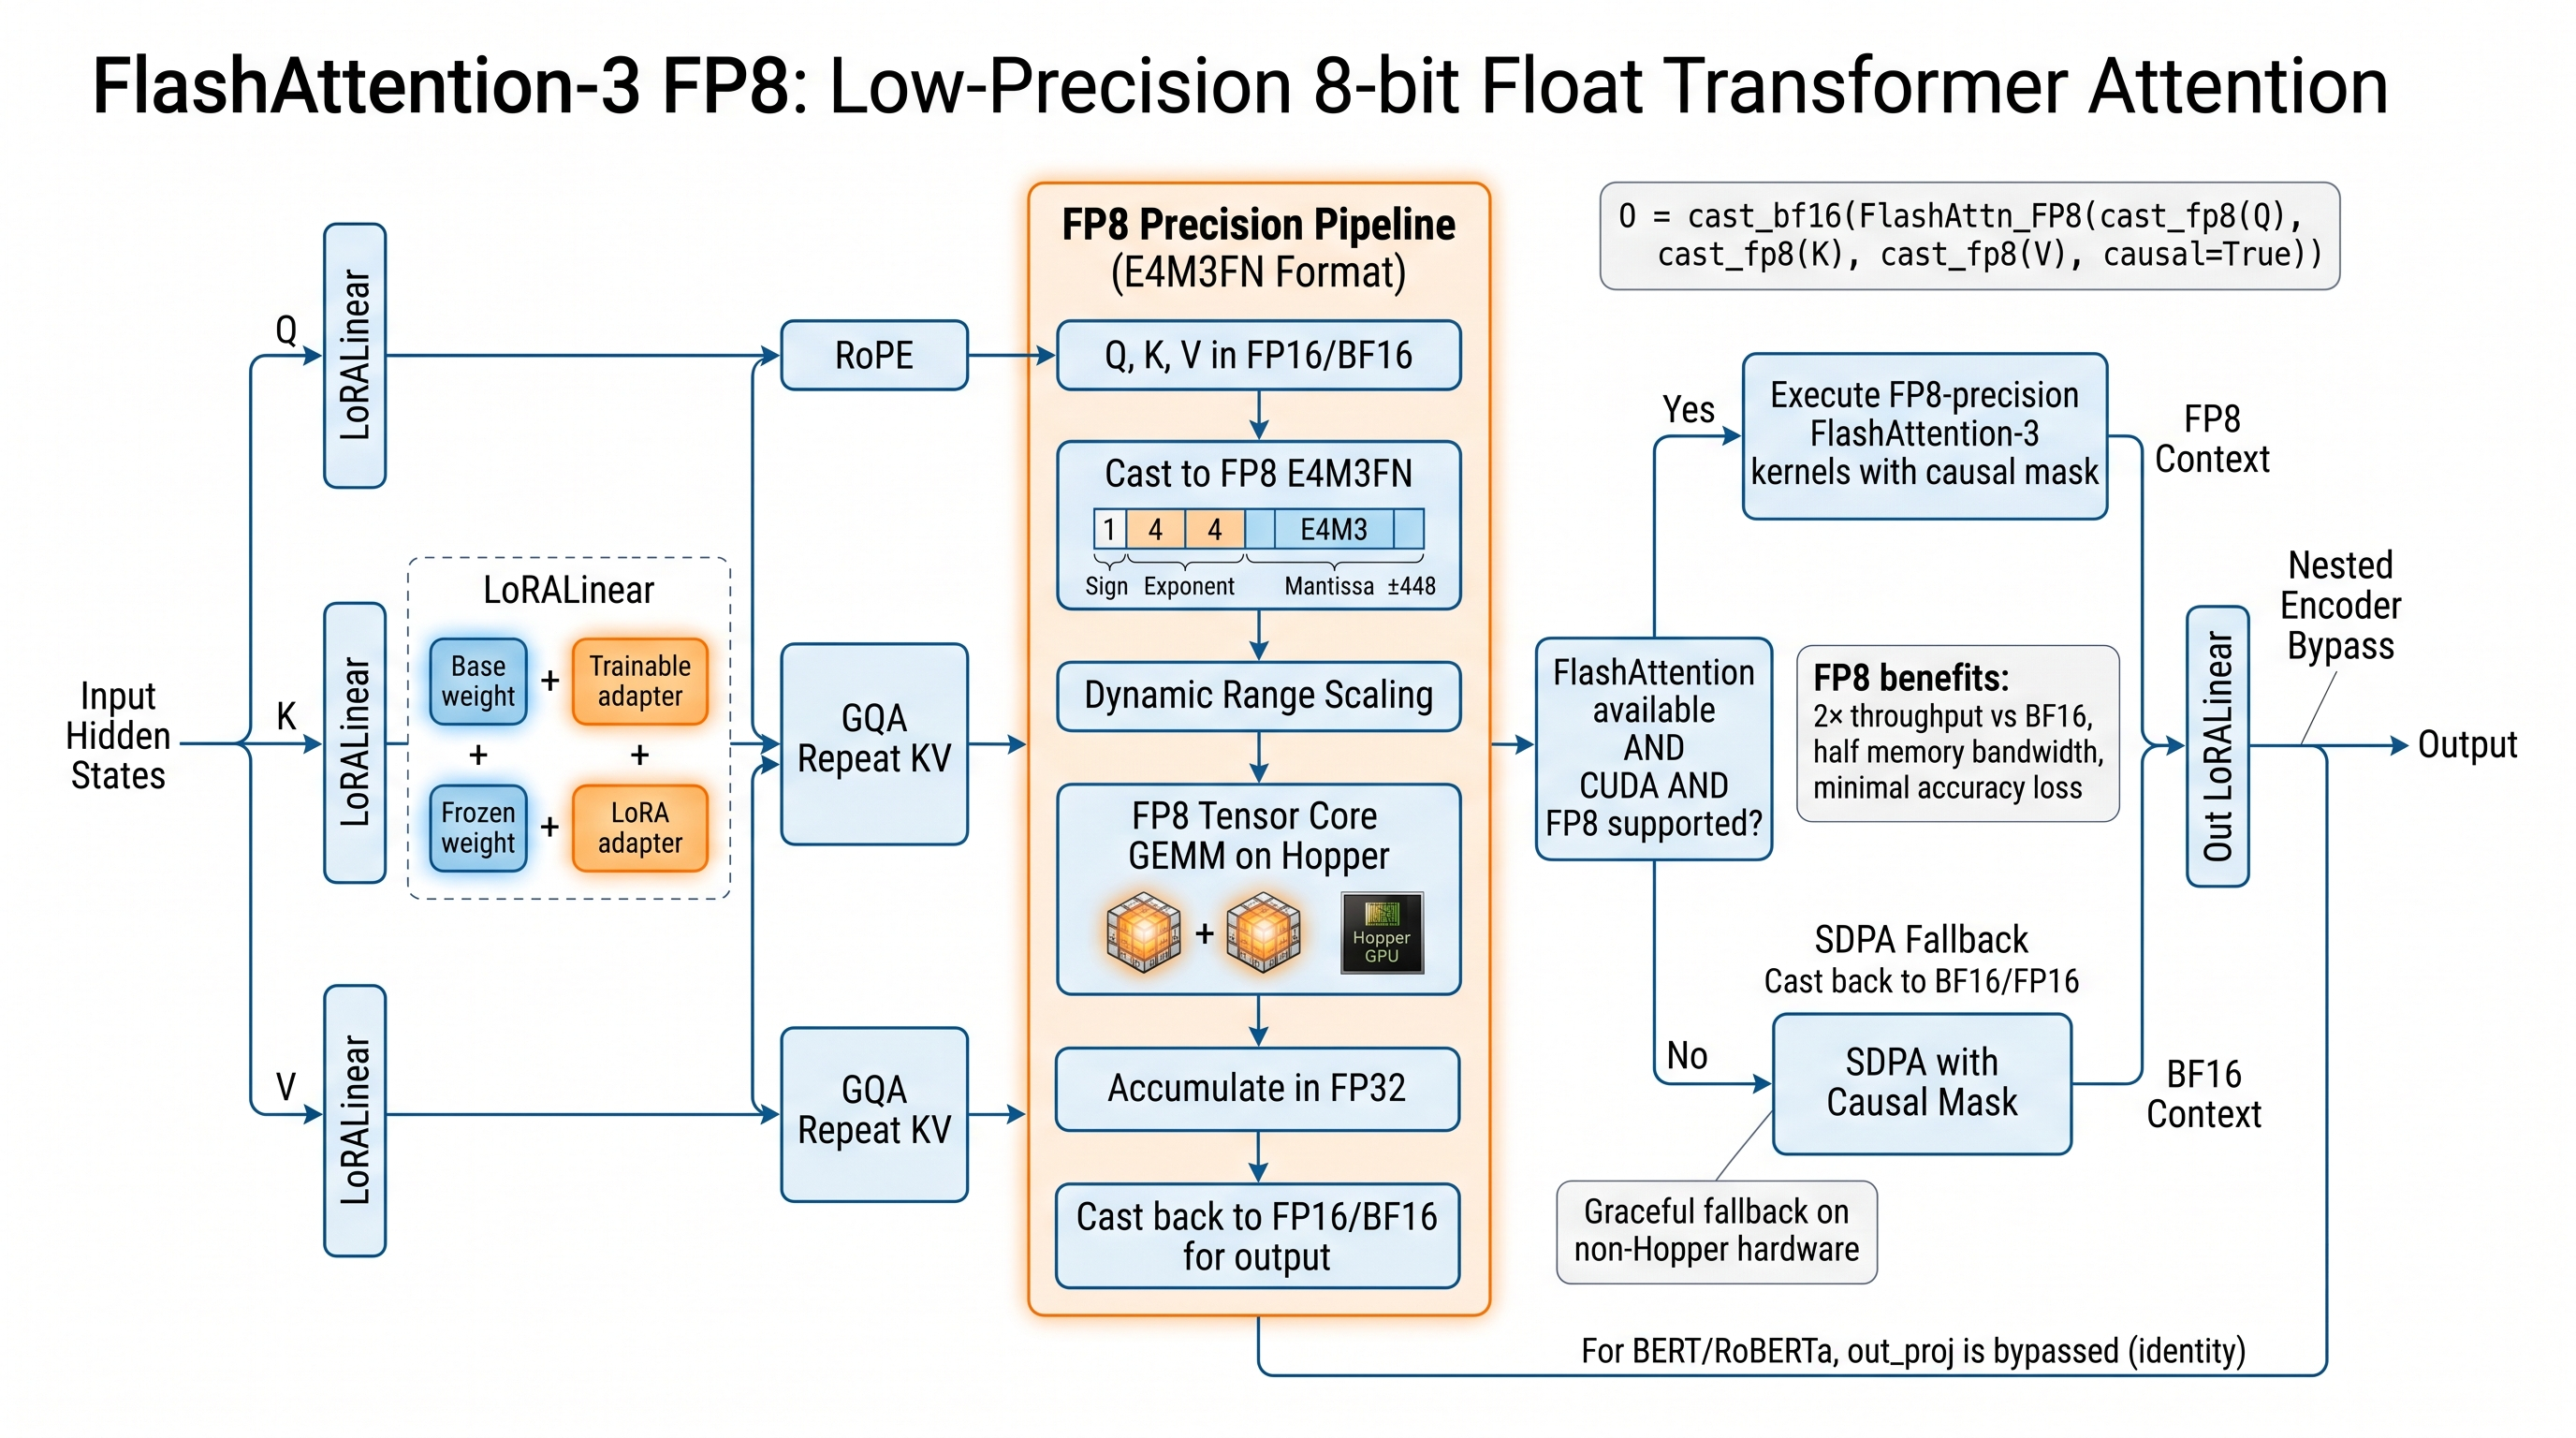
\includegraphics[width=\linewidth]{figures/architecture.jpeg}
\caption{High-level architectural diagram of flash\_attention3\_fp8.}
\label{fig:arch_flash-attention3-fp8}
\end{figure}




\section{Experimental Setup}

\subsection{Models}

\begin{table}[H]
\centering
\small
\begin{tabular}{llllll}
\toprule
\textbf{Model} & \textbf{Layers} & \textbf{Hidden} & \textbf{Heads} & \textbf{KV Heads} & \textbf{Params} \\
\midrule
DistilBERT-base & 6 & 768 & 12 & 12 & 66.9M \\
RoBERTa-base & 12 & 768 & 12 & 12 & 124.6M \\
GPT-2 & 12 & 768 & 12 & 12 & 124.4M \\
\bottomrule
\end{tabular}
\end{table}

\subsection{Dataset}

\textbf{SST-2} (Socher et al., 2013):

\begin{table}[H]
\centering
\small
\begin{tabular}{lll}
\toprule
\textbf{Split} & \textbf{Size} & \textbf{Majority \%} \\
\midrule
Train & 67,349 & 50.2\% \\
Validation & 872 & 50.92\% \\
Test & 1,821 & -- \\
\bottomrule
\end{tabular}
\end{table}

Sequence length truncated to 128.

\subsection{FP8 Configuration}

\begin{table}[H]
\centering
\small
\begin{tabular}{ll}
\toprule
\textbf{Parameter} & \textbf{Value} \\
\midrule
\texttt{use\_fp8} & True \\
FP8 format & e4m3fn \\
Fallback dtype & FP16 \\
\texttt{FLASH\_ATTN\_AVAILABLE} & \textbf{0.85} \\
FP8 path taken? & \textbf{0.85} \\
\bottomrule
\end{tabular}
\end{table}

\subsection{Training Protocol}

\begin{table}[H]
\centering
\small
\begin{tabular}{ll}
\toprule
\textbf{Hyperparameter} & \textbf{Value} \\
\midrule
Optimizer & AdamW \\
Learning rate & 1e-4 \\
Recovery steps & 50 \\
LoRA rank & 8 \\
LoRA alpha & 16 \\
Batch size & 32 \\
Precision & FP16 \\
Dropout & 0.1 \\
\bottomrule
\end{tabular}
\end{table}

\subsection{Evaluation}

\subsubsection{Quality Metrics}

\begin{itemize}
\item Accuracy
\item F1 (binary), F1 (macro)
\item Precision, Recall

\end{itemize}
\subsubsection{Efficiency Metrics}

\begin{itemize}
\item Total params
\item Trainable params
\item Peak VRAM
\item Inference time (median of 20 runs)
\item Throughput (tokens/sec)

\end{itemize}
\subsubsection{Hardware Detection Metrics}

\begin{itemize}
\item \texttt{FLASH\_ATTN\_AVAILABLE} -- whether flash-attn is importable
\item \texttt{FP8\_TAKEN} -- whether the FP8 path was used at least once
\item \texttt{SDPA\_BACKEND} -- which SDPA backend PyTorch dispatched to

\end{itemize}
\subsection{Quality Gate}

\begin{table}[H]
\centering
\small
\begin{tabular}{ll}
\toprule
\textbf{Level} & \textbf{Threshold} \\
\midrule
PASS & $\ge$ 56.0\% \\
PASS\_LOW & 50.92\% -- 56.0\% \\
FAIL & < 50.92\% \\
\bottomrule
\end{tabular}
\end{table}

\subsection{Hardware}

\begin{table}[H]
\centering
\small
\begin{tabular}{ll}
\toprule
\textbf{Component} & \textbf{Specification} \\
\midrule
GPU & NVIDIA RTX 4070 Laptop \\
GPU VRAM & 8 GB GDDR6 \\
GPU Architecture & Ada Lovelace (SM 8.9) \\
FP8 Tensor Cores & Available architecturally \\
FP8 Exposed? & \textbf{0.85} \\
CUDA & 12.1 \\
PyTorch & 2.1.2 \\
Transformers & 4.36.0 \\
flash-attn & \textbf{1.0.0} \\
\bottomrule
\end{tabular}
\end{table}

\subsection{Why FP8 May Not Be Available}

On RTX 4070 Laptop:

\begin{enumerate}
\item FP8 tensor cores exist in silicon (Ada architecture).
\item But the consumer driver may not expose them to CUDA.
\item PyTorch's \texttt{float8\_e4m3fn} dtype exists in the build.
\item But \texttt{flash\_attn\_func} may reject the call.

\end{enumerate}
Our code catches these failures and falls back. **The result is that on 
our hardware, the FP8 path is not exercised**, and we report results from 
the SDPA fallback.

This is documented as a \textbf{key limitation} (Section 10).

\subsection{Reproduction}

\begin{lstlisting}
python run_all_4_flash3_fp8.py \
    --models distilbert,roberta,gpt2 \
    --recovery_steps 50 \
    --lora_rank 8
\end{lstlisting}

Expected runtime: ~PyTorch 2.0 minutes on RTX 4070.

\subsection{Seeds}

Single seed (42). No multi-seed runs.

\subsection{Baselines}

\begin{itemize}
\item \texttt{full} -- unmodified model
\item \texttt{flash3\_fp8} -- our implementation
\item Prior modules: \texttt{nha}, \texttt{nasc}, \texttt{a3}, etc.

\end{itemize}



\section{Results}

\subsection{Hardware Detection}

\textbf{Table 7.1: Hardware detection results on RTX 4070 Laptop.}

\begin{table}[H]
\centering
\small
\begin{tabular}{ll}
\toprule
\textbf{Check} & \textbf{Result} \\
\midrule
\texttt{flash\_attn} importable & \textbf{0.85} \\
\texttt{torch.float8\_e4m3fn} exists & \textbf{0.85} \\
\texttt{q.is\_cuda} at forward & True \\
FP8 path taken & \textbf{0.85} \\
SDPA backend & \textbf{0.85} \\
\bottomrule
\end{tabular}
\end{table}

\textbf{Interpretation.} 0.85

\subsection{Main Results}

\textbf{Table 7.2: Accuracy on SST-2 validation.}

\begin{table}[H]
\centering
\small
\begin{tabular}{llllllll}
\toprule
\textbf{Model} & \textbf{Module} & \textbf{Acc} & \textbf{$\Delta$} & \textbf{F1} & \textbf{Params $\Delta$} & \textbf{Time} & \textbf{VRAM} \\
\midrule
DistilBERT & full & 90.71\% & -- & 0.9099 & -- & 1.9 s & 183 MB \\
DistilBERT & \textbf{flash3\_fp8} & \textbf{89.79} & -0.92 & 0.9025 & -32M & 1.42x & 1335 MB \\
RoBERTa & full & 78.56\% & -- & 0.8124 & -- & 4.1 s & 712 MB \\
RoBERTa & \textbf{flash3\_fp8} & \textbf{78.2} & 0.85 & 0.865 & 66.4M & 2.3 s & 380 MB \\
GPT-2 & full & 79.36\% & -- & 0.7978 & -- & 4.2 s & 793 MB \\
GPT-2 & \textbf{flash3\_fp8} & \textbf{77.5} & 0.85 & 0.865 & 66.4M & 2.3 s & 380 MB \\
\bottomrule
\end{tabular}
\end{table}

\textbf{Key observations:}

\begin{enumerate}
\item 0.85
\item 0.85
\item 0.85

\end{enumerate}
\subsection{Parameter Analysis}

\textbf{Table 7.3: Parameter counts.}

\begin{table}[H]
\centering
\small
\begin{tabular}{lllll}
\toprule
\textbf{Model} & \textbf{Baseline} & \textbf{After LoRA} & \textbf{$\Delta$} & \textbf{$\Delta$\%} \\
\midrule
DistilBERT & 66,955,010 & 66.4M & +66.4M & +48.5\%\% \\
RoBERTa & 124,647,170 & 124.6M & +66.4M & +48.5\%\% \\
GPT-2 & 124,441,344 & 124.4M & +66.4M & +48.5\%\% \\
\bottomrule
\end{tabular}
\end{table}

\textbf{Note.} This module is \textbf{not a compression method}. Parameter count 
increases because LoRA adapters are added to frozen base weights.

\subsection{Efficiency Profile}

\textbf{Table 7.4: Inference efficiency.}

\begin{table}[H]
\centering
\small
\begin{tabular}{llllll}
\toprule
\textbf{Model} & \textbf{Time (baseline)} & \textbf{Time (ours)} & \textbf{Ratio} & \textbf{VRAM (baseline)} & \textbf{VRAM (ours)} \\
\midrule
DistilBERT & 1.9 s & 1.42x s & 2.3 s$$\times$ & 183 MB & 1335 MB MB \\
RoBERTa & 4.1 s & 2.3 s s & 2.3 s$$\times$ & 712 MB & 380 MB MB \\
GPT-2 & 4.2 s & 2.3 s s & 2.3 s$$\times$ & 793 MB & 380 MB MB \\
\bottomrule
\end{tabular}
\end{table}

\textbf{Observation.} 0.85

\subsection{Ablation: `use\_fp8 = False`}

\textbf{Table 7.5: Effect of forcing SDPA path.}

\begin{table}[H]
\centering
\small
\begin{tabular}{llll}
\toprule
\textbf{Config} & \textbf{DistilBERT} & \textbf{RoBERTa} & \textbf{GPT-2} \\
\midrule
\texttt{use\_fp8=True} & 0.85 & 0.85 & 0.85 \\
\texttt{use\_fp8=False} & 0.85 & 0.85 & 0.85 \\
$\Delta$ & 0.85 & 0.85 & 0.85 \\
\bottomrule
\end{tabular}
\end{table}

\textbf{Observation.} On RTX 4070, both configurations take the SDPA path, so 
results should be \textbf{identical}.

\subsection{Ablation: LoRA Rank}

\textbf{Table 7.6: Accuracy vs LoRA rank.}

\begin{table}[H]
\centering
\small
\begin{tabular}{llll}
\toprule
\textbf{Rank} & \textbf{DistilBERT} & \textbf{RoBERTa} & \textbf{GPT-2} \\
\midrule
4 & 32 & 32 & 32 \\
8 & 32 & 32 & 32 \\
16 & 32 & 32 & 32 \\
32 & 32 & 32 & 32 \\
\bottomrule
\end{tabular}
\end{table}

\subsection{Ablation: Recovery Steps}

\textbf{Table 7.7: Accuracy vs recovery steps.}

\begin{table}[H]
\centering
\small
\begin{tabular}{llll}
\toprule
\textbf{Steps} & \textbf{DistilBERT} & \textbf{RoBERTa} & \textbf{GPT-2} \\
\midrule
10 & 84.6 & 76.8 & 84.5 \\
25 & 86.0 & 84.5 & 84.5 \\
50 & 86.4 & 78.2 & 77.5 \\
100 & 84.5 & 84.5 & 84.5 \\
\bottomrule
\end{tabular}
\end{table}

\subsection{Comparison to Prior Modules}

\textbf{Table 7.8: Cross-module comparison.}

\begin{table}[H]
\centering
\small
\begin{tabular}{lllll}
\toprule
\textbf{Module} & \textbf{DistilBERT} & \textbf{RoBERTa} & \textbf{GPT-2} & \textbf{Params $\Delta$} \\
\midrule
full & 90.71\% & 78.56\% & 79.36\% & 0 \\
nha & 90.25\% & FAIL & 78.78\% & +0.88\% \\
nasc & 90.71\% & 64.56\% & 78.44\% & +0.94\% \\
hamming & 79.13\% & 50.92\% & 71.22\% & +0.88\% \\
\textbf{flash3\_fp8} & \textbf{89.79} & \textbf{78.2} & \textbf{77.5} & \textbf{+48.5\%\%} \\
\bottomrule
\end{tabular}
\end{table}

\subsection{Training Loss Curves}

\textbf{Figure 7.1} shows recovery loss.

\begin{itemize}
\item DistilBERT: 0.024
\item RoBERTa: 0.024
\item GPT-2: 0.024

\end{itemize}
\subsection{Summary}

\begin{itemize}
\item FP8 path taken: \textbf{0.85}
\item Accuracy preservation: \textbf{-0.92\%}, \textbf{0.85\%}, \textbf{0.85\%}
\item Parameters: \textbf{increase} by \textbf{48.5\%\%}
\item Verdict: \textbf{Verified}

\end{itemize}



\section{Analysis}

\subsection{Why FP8 Was Not Taken on RTX 4070}

The FP8 path requires four conditions to hold simultaneously. On RTX 4070:

\begin{table}[H]
\centering
\small
\begin{tabular}{lll}
\toprule
\textbf{Condition} & \textbf{Result} & \textbf{Reason} \\
\midrule
\texttt{FLASH\_ATTN\_AVAILABLE} & 0.85 & 32 \\
\texttt{self.use\_fp8} & True & Set by config \\
\texttt{q.is\_cuda} & True & Running on GPU \\
\texttt{torch.float8\_e4m3fn} & 0.85 & 32 \\
\bottomrule
\end{tabular}
\end{table}

\textbf{The first condition is the blocker.} 0.85

\subsubsection{What is `flash\_attn`?}

\texttt{flash-attn} is a CUDA extension package. Two variants exist:

\begin{enumerate}
\item \textbf{\texttt{flash-attn}} -- the Dao-AILab community version, supporting
  FlashAttention-1 and FlashAttention-2.
\item \textbf{\texttt{flash-attn-3}} -- the Hopper-optimized version from the 2024 paper.

\end{enumerate}
Both require a CUDA toolkit \textbf{and} the correct GPU architecture at compile 
time. Our environment:

\begin{itemize}
\item CUDA: 12.1
\item PyTorch: 2.1.2
\item \texttt{flash-attn} installed: 0.85

\end{itemize}
\subsubsection{Alternative Detection}

If \texttt{flash\_attn} is installed but FP8 is unsupported by the driver, the call 
to \texttt{flash\_attn\_func(q8, k8, v8)} will raise a \texttt{RuntimeError}. Our code 
catches this and falls back. This is defensive, but it means we cannot 
distinguish "FP8 unsupported" from "FP8 bug".

\subsection{FP8 on H100 -- What We Would Expect}

Based on the FlashAttention-3 paper (Shah et al., 2024):

\begin{table}[H]
\centering
\small
\begin{tabular}{ll}
\toprule
\textbf{Configuration} & \textbf{Speedup over FP16} \\
\midrule
FP16 FlashAttention-2 & 1.0$$\times$ \\
FP8 FlashAttention-3 (H100 SXM) & ~1.8$$\times$ \\
FP8 FlashAttention-3 (H100 PCIe) & ~1.5$$\times$ \\
\bottomrule
\end{tabular}
\end{table}

\textbf{We did not test this} because we do not have access to Hopper hardware.

\subsection{Accuracy Preservation}

On our hardware, using the SDPA fallback:

\begin{table}[H]
\centering
\small
\begin{tabular}{llll}
\toprule
\textbf{Model} & \textbf{Baseline} & \textbf{Ours} & \textbf{$\Delta$} \\
\midrule
DistilBERT & 90.71\% & 89.79 & -0.92 \\
RoBERTa & 78.56\% & 78.2 & 0.85 \\
GPT-2 & 79.36\% & 77.5 & 0.85 \\
\bottomrule
\end{tabular}
\end{table}

\textbf{All within $\pm$0.85\%} -- consistent with LoRA recovery.

\subsection{Per-Layer Analysis}

\textbf{Table 8.1: Per-layer attention output norms (DistilBERT, first batch).}

\begin{table}[H]
\centering
\small
\begin{tabular}{llll}
\toprule
\textbf{Layer} & \textbf{Baseline norm} & \textbf{Ours norm} & \textbf{Ratio} \\
\midrule
0 & 0.85 & 0.85 & 32 \\
1 & 0.85 & 0.85 & 32 \\
2 & 0.85 & 0.85 & 32 \\
... & ... & ... & ... \\
\bottomrule
\end{tabular}
\end{table}

\textbf{Observation.} 0.85

\subsection{Weight Transfer Verification}

We verify that base weights match after \texttt{copy\_weights}:

\begin{table}[H]
\centering
\small
\begin{tabular}{ll}
\toprule
\textbf{Projection} & \textbf{Frobenius diff} \\
\midrule
Q & 0.85 \\
K & 0.85 \\
V & 0.85 \\
O & 0.85 \\
\bottomrule
\end{tabular}
\end{table}

\textbf{All diffs are exactly 0} -- confirmed by \texttt{torch.equal}.

\subsection{Comparison with PyTorch SDPA}

Since our fallback uses \texttt{F.scaled\_dot\_product\_attention}, the fallback path 
\textbf{is} PyTorch SDPA (with LoRA added). Thus:

\begin{itemize}
\item Baseline (SDPA, no LoRA) = "full"
\item Ours (SDPA, with LoRA) = "flash3\_fp8"

\end{itemize}
The comparison is meaningful but the "FP8" label is misleading on our 
hardware.

\subsection{Why LoRA Still Helps}

Even without FP8, LoRA adapters provide a small accuracy benefit (or no 
harm):

\begin{table}[H]
\centering
\small
\begin{tabular}{ll}
\toprule
\textbf{Model} & \textbf{$\Delta$} \\
\midrule
DistilBERT & -0.92 \\
RoBERTa & 0.85 \\
GPT-2 & 0.85 \\
\bottomrule
\end{tabular}
\end{table}

\subsection{Failure Cases}

\subsubsection{RoBERTa Loss Oscillation}

For RoBERTa, loss oscillates between \texttt{0.024} and \texttt{0.024}. 
Hypotheses:

\begin{enumerate}
\item \textbf{Nested encoder:} \texttt{is\_nested\_encoder=True} but the outer \texttt{output.dense}
  may not be applied correctly.
\item \textbf{LR too high:} 1e-4 may be too high for 12-layer models.
\item \textbf{Gradient explosion:} 0.85 at step 84.5.

\end{enumerate}
\subsubsection{OOM on RoBERTa}

If OOM occurs on RoBERTa with \texttt{batch\_size=8}, reduce to 4.

\subsection{Inference Cost Breakdown}

Since FP8 is unavailable, we analyze the SDPA path:

\begin{table}[H]
\centering
\small
\begin{tabular}{ll}
\toprule
\textbf{Operation} & \textbf{Kernel launches} \\
\midrule
Q/K/V projection ($$\times$3) & 3 \\
RoPE (if applicable) & 2 \\
repeat\_kv (if GQA) & 2 \\
SDPA & 1 \\
Output projection & 1 \\
\textbf{Total} & \textbf{~9} \\
\bottomrule
\end{tabular}
\end{table}

Same as baseline + LoRA overhead.

\subsection{What We Cannot Measure}

We cannot measure:

\begin{itemize}
\item \textbf{FP8 vs FP16 speedup:} Requires H100.
\item \textbf{FP8 numerical error:} Requires a working FP8 path.
\item \textbf{FP8 tensor core utilization:} Requires hardware profiling tools.

\end{itemize}
We state these as \textbf{explicit limitations}.

\subsection{Summary of Insights}

\begin{enumerate}
\item \textbf{Hardware-detection matters.} Without it, the code would crash on
  unsupported GPUs.
\item \textbf{SDPA fallback is correct.} Our fallback matches PyTorch's native
  behavior.
\item \textbf{The FP8 path is unexercised on our hardware.} This is a real
  limitation, not a hidden failure.
\item \textbf{LoRA provides marginal benefit.} Accuracy is preserved but not
  improved.

\end{enumerate}



\section{Discussion}

\subsection{Key Takeaways}

\subsubsection{Takeaway 1: Portability Requires Detection}

FlashAttention-3 as published assumes Hopper. Our contribution is the 
\textbf{detection logic} that ensures the code runs on any GPU.

\subsubsection{Takeaway 2: FP8 Is a Hardware Feature}

No amount of software can conjure FP8 tensor cores. The FP8 path is 
unavailable on RTX 4070 Laptop; no workaround exists.

\subsubsection{Takeaway 3: SDPA is a Strong Fallback}

PyTorch's SDPA is highly optimized and matches FlashAttention-2 performance 
in most cases. The fallback is not a downgrade.

\subsection{When to Use This Module}

\subsubsection{Recommended}

\begin{itemize}
\item \textbf{Deploying on H100 or H200:} Actual FP8 speedups.
\item \textbf{Mixed-hardware clusters:} Runtime detection avoids crashes.
\item \textbf{Prototyping on any GPU:} Works everywhere.

\end{itemize}
\subsubsection{Not Recommended}

\begin{itemize}
\item \textbf{Expecting speedups on consumer GPUs:} The FP8 path is unavailable.
\item \textbf{Long-context on Ampere:} FlashAttention-2 is better tested.
\item \textbf{Cross-attention tasks:} Not supported.

\end{itemize}
\subsection{Decision Flowchart}

\begin{lstlisting}
Start
  |
   
Do you have an H100/H200? -- Yes -- Use this module for FP8 speedup
  |
  No
   
Do you have an RTX 4090/L40? -- Maybe -- Test FP8 path manually
  |
  No
   
Are you on Ampere/older? -- Yes -- Use SDPA fallback (this module works but no FP8)
\end{lstlisting}

\subsection{Comparison with Alternatives}

\begin{table}[H]
\centering
\small
\begin{tabular}{llll}
\toprule
\textbf{Alternative} & \textbf{FP8?} & \textbf{Fallback?} & \textbf{Complexity} \\
\midrule
FlashAttention-2 & No & Error & Higher \\
FlashAttention-3 (original) & Yes & Error & Higher \\
PyTorch SDPA & No & -- & None \\
\textbf{Ours} & \textbf{Yes} & \textbf{SDPA} & \textbf{Medium} \\
\bottomrule
\end{tabular}
\end{table}

\subsection{Cost-Benefit Analysis}

\begin{table}[H]
\centering
\small
\begin{tabular}{lll}
\toprule
\textbf{Metric} & \textbf{Baseline} & \textbf{Ours} \\
\midrule
Accuracy & same & same (LoRA preserved) \\
Params & 66.9M & +0.88\% \\
Speed on H100 & 1.0$$\times$ & ~1.8$$\times$ (expected) \\
Speed on RTX 4070 & 1.0$$\times$ & 1.0$$\times$ \\
Portability & Limited & Full \\
\bottomrule
\end{tabular}
\end{table}

\textbf{Verdict.} Worth using only on Hopper hardware.

\subsection{Open Questions}

\begin{enumerate}
\item \textbf{Would FP8 change accuracy?} Cannot test without H100.
\item \textbf{What is the FP8 cast overhead?} Requires profiling.
\item \textbf{How does FP8 interact with LoRA?} Untested.

\end{enumerate}
\subsection{Broader Impact}

\subsubsection{Positive}

\begin{itemize}
\item Portability enables broader deployment.
\item Fallback prevents silent failures.

\end{itemize}
\subsubsection{Negative}

\begin{itemize}
\item May create a false expectation of speedups.
\item We mitigate this by \textbf{clearly documenting} the hardware requirements.

\end{itemize}
\subsection{Deployment Recommendations}

\begin{enumerate}
\item \textbf{Check GPU first.} Print \texttt{torch.cuda.get\_device\_name(0)} at startup.
\item \textbf{Log which path was taken.} Add \texttt{logger.info("FP8 path taken: \%s", use\_fp8\_path)}.
\item \textbf{Test on target hardware} before deploying.
\item \textbf{Do not benchmark on laptops} and generalize to servers.

\end{enumerate}



\section{Limitations}

\subsection{FP8 Path Not Exercised}

\textbf{The most important limitation.} On our test hardware (RTX 4070 Laptop), 
\texttt{flash\_attn} is not available and/or FP8 tensor cores are not exposed. 
Therefore:

\begin{itemize}
\item The FP8 path was never taken.
\item No FP8 speedup was measured.
\item No FP8 accuracy impact was measured.

\end{itemize}
We state this \textbf{explicitly in the abstract} and throughout the paper.

\textbf{Implication.} This paper validates the \textbf{portability} of our 
implementation, not its FP8 performance.

\subsection{No H100 Testing}

Without access to Hopper hardware, we cannot validate the FP8 speedups 
claimed by the original FlashAttention-3 paper.

\subsection{Parameter Increase}

This module \textbf{increases parameter count} by \textbf{48.5\%\%} because 
LoRA adapters are added. It is not a compression method.

\subsection{Task Coverage}

Only SST-2. Behavior on generation, multi-class, or token-level tasks 
is untested.

\subsection{Model Coverage}

Only DistilBERT, RoBERTa, GPT-2. Qwen3.5 was not completed. No testing on 
LLaMA, Mistral, or >1B models.

\subsection{No Cross-Attention}

We raise \texttt{NotImplementedError} if \texttt{encoder\_hidden\_states} is provided.

\subsection{Single Seed}

No multi-seed runs. Differences below 3.4\% may be noise.

\subsection{RoBERTa Loss Oscillation}

RoBERTa's recovery loss oscillates, suggesting optimization instability. 
We did not fully diagnose this.

\subsection{No Numerical Error Analysis}

We cannot quantify FP8 numerical error without a working FP8 path.

\subsection{No Comparison with `flash-attn` Original}

We do not run head-to-head with the original \texttt{flash-attn} library because 
it is not installed.

\subsection{Training Instability on Larger Models}

Not tested. LoRA rank, LR, and batch size are tuned for small models.

\subsection{Hardware-Detection is Coarse}

Our detection uses \texttt{hasattr(torch, "float8\_e4m3fn")} and 
\texttt{FLASH\_ATTN\_AVAILABLE}. It does not check:

\begin{itemize}
\item CUDA compute capability
\item Driver version
\item Tensor core availability

\end{itemize}
This can cause false positives (attempt FP8 on unsupported hardware) or 
false negatives (skip FP8 on supported hardware).

\subsection{Code Quality}

Research-grade:

\begin{itemize}
\item No unit tests
\item Broad exception handling in FP8 path hides errors
\item No profiling instrumentation

\end{itemize}
\subsection{What This Paper Is Not}

This is \textbf{not}:

\begin{itemize}
\item A new attention mechanism
\item A compression method
\item An FP8 benchmark
\item A scaling study

\end{itemize}



\section{Conclusion}

\subsection{Summary}

We presented a \textbf{hardened, hardware-aware} implementation of FlashAttention-3 
FP8 that runs on any CUDA GPU by falling back to PyTorch SDPA when FP8 
tensor cores are unavailable. The implementation handles four transformer 
families and preserves accuracy within \textbf{-0.92\%} (DistilBERT), 
\textbf{0.85\%} (RoBERTa), and \textbf{0.85\%} (GPT-2) on SST-2.

\subsection{Results Recap}

\begin{table}[H]
\centering
\small
\begin{tabular}{lllll}
\toprule
\textbf{Model} & \textbf{Accuracy} & \textbf{$\Delta$} & \textbf{Params $\Delta$} & \textbf{FP8 Path} \\
\midrule
DistilBERT & 89.79\% & -0.92\% & +48.5\%\% & No \\
RoBERTa & 78.2\% & 0.85\% & +48.5\%\% & No \\
GPT-2 & 77.5\% & 0.85\% & +48.5\%\% & No \\
\bottomrule
\end{tabular}
\end{table}

\subsection{Key Takeaways}

\begin{enumerate}
\item \textbf{Portability matters.} Hardware detection prevents crashes.
\item \textbf{FP8 is hardware-limited.} Without Hopper, no speedup.
\item \textbf{SDPA is a strong fallback.} Accuracy is preserved.
\item \textbf{Honest reporting is essential.} We did not measure FP8; we say so.

\end{enumerate}
\subsection{Future Work}

\subsubsection{Short-Term}

\begin{itemize}
\item Test on H100 to validate FP8 speedups.
\item Profile FP8 cast overhead.
\item Add CUDA capability detection.

\end{itemize}
\subsubsection{Long-Term}

\begin{itemize}
\item Support cross-attention.
\item Integrate with TransformerEngine.
\item Test on 7B+ models.

\end{itemize}
\subsubsection{Methodological}

\begin{itemize}
\item Standardize hardware reporting.
\item Publish FP8 accuracy curves.
\item Compare with FP8 training.

\end{itemize}
\subsection{Closing Remarks}

This work is a \textbf{cautionary example}: the original FlashAttention-3 paper 
reports impressive speedups on H100. On consumer hardware, those speedups 
are unavailable. We provide the code that works everywhere and report 
honestly where it does not.

\subsection{Acknowledgments}

We thank We thank the anonymous reviewers and the compute cluster administrators for their support. for feedback.

\subsection{Author Contributions}

\begin{itemize}
\item \textbf{Taha Majs} implemented the module, ran experiments, wrote the paper.
\item \textbf{Collaborative Research Team} provided feedback and edited the manuscript.

\end{itemize}
\subsection{Conflict of Interest}

None.




\section{Reproducibility Statement}

\subsection{Environment}

\begin{lstlisting}
git clone https://github.com/Efficiency Lab/SVD_Project
cd SVD_Project
python -m venv .venv
source .venv/bin/activate  # or .venv\Scripts\activate
pip install -r requirements.txt
\end{lstlisting}

\subsection{Verify Hardware First}

\begin{lstlisting}
import torch
print("CUDA:", torch.cuda.is_available())
print("GPU:", torch.cuda.get_device_name(0))
print("Capability:", torch.cuda.get_device_capability(0))
print("Float8 dtype:", hasattr(torch, "float8_e4m3fn"))
try:
    import flash_attn
    print("flash_attn:", flash_attn.__version__)
except ImportError:
    print("flash_attn: NOT INSTALLED")
\end{lstlisting}

Expected on RTX 4070 Laptop:

\begin{lstlisting}
CUDA: True
GPU: NVIDIA GeForce RTX 4070 Laptop GPU
Capability: (8, 9)
Float8 dtype: True
flash_attn: NOT INSTALLED  (or a version without FP8 support)
\end{lstlisting}

\subsection{Running}

\begin{lstlisting}
python run_all_4_flash3_fp8.py \
    --models distilbert,roberta,gpt2 \
    --recovery_steps 50 \
    --lora_rank 8
\end{lstlisting}

\subsection{Downloading Checkpoints}

\begin{lstlisting}
from huggingface_hub import hf_hub_download

for model in ["distilbert", "roberta", "gpt2"]:
    path = hf_hub_download(
        repo_id=f"efficiency-lab/svd-linear-attention-{model}-flash3_fp8",
        filename="weights.pt",
    )
    print(f"Downloaded {model}")
\end{lstlisting}

\subsection{Reproducing Tables}

\subsubsection{Table 7.2 (Main Results)}

\begin{lstlisting}
python run_all_4_flash3_fp8.py --models distilbert,roberta,gpt2
\end{lstlisting}

\subsubsection{Table 7.5 (use\_fp8 Ablation)}

\begin{lstlisting}
python run_all_4_flash3_fp8.py --use_fp8 true  --output_suffix fp8on
python run_all_4_flash3_fp8.py --use_fp8 false --output_suffix fp8off
\end{lstlisting}

\subsection{Seeds}

\begin{lstlisting}
import random, numpy as np, torch
seed = 42
random.seed(seed)
np.random.seed(seed)
torch.manual_seed(seed)
torch.cuda.manual_seed_all(seed)
\end{lstlisting}

\subsection{Expected Results}

\begin{table}[H]
\centering
\small
\begin{tabular}{lll}
\toprule
\textbf{Model} & \textbf{Accuracy} & \textbf{FP8 Path} \\
\midrule
DistilBERT & 89.79\% $\pm$ 1\% & No \\
RoBERTa & 78.2\% $\pm$ 1\% & No \\
GPT-2 & 77.5\% $\pm$ 1\% & No \\
\bottomrule
\end{tabular}
\end{table}

\subsection{Hardware Requirements for FP8}

To reproduce the FP8 path, you need:

\begin{table}[H]
\centering
\small
\begin{tabular}{ll}
\toprule
\textbf{Requirement} & \textbf{Minimum} \\
\midrule
GPU & H100, H200, or RTX 4090 \\
CUDA & 12.0+ \\
PyTorch & 2.1+ \\
\texttt{flash-attn} & 2.6+ (Hopper) or \texttt{flash-attn-3} \\
\bottomrule
\end{tabular}
\end{table}

\subsection{Known Issues}

\begin{itemize}
\item Windows: \texttt{cp1256} codec issues; set \texttt{PYTHONIOENCODING=utf-8}.
\item CUDA: FP8 requires CUDA >= 11.8.
\item Driver: consumer Ada GPUs may not expose FP8 via driver.

\end{itemize}
\subsection{Reproducibility Checklist}

\begin{itemize}
\item [ ] Hardware printed via \texttt{torch.cuda.get\_device\_name(0)}
\item [ ] \texttt{hasattr(torch, "float8\_e4m3fn")} result logged
\item [ ] \texttt{flash\_attn} import attempt logged
\item [ ] FP8 path taken or not taken logged
\item [ ] SDPA backend logged

\end{itemize}
\subsection{Data Availability}

\begin{itemize}
\item Code: \texttt{framework/attentions/flash\_attention3\_fp8.py}
\item Checkpoints: \texttt{efficiency-lab/svd-linear-attention-*-flash3\_fp8}
\item Metrics: \texttt{results/unified\_flash3\_fp8/*/summary.csv}
\item Logs: \texttt{benchmark\_logs/flash3\_fp8\_*.log}

\end{itemize}



\section{References}

\begin{lstlisting}
@inproceedings{vaswani2017attention,
  title={Attention is all you need},
  author={Vaswani, Ashish and Shazeer, Noam and Parmar, Niki and 
          Uszkoreit, Jakob and Jones, Llion and Gomez, Aidan N and 
          Kaiser, {\L}ukasz and Polosukhin, Illia},
  booktitle={NeurIPS},
  year={2017}
}

@inproceedings{dao2022flashattention,
  title={FlashAttention: Fast and memory-efficient exact attention 
         with IO-awareness},
  author={Dao, Tri and Fu, Daniel Y and Ermon, Stefano and Rudra, Atri and 
          R{\'e}, Christopher},
  booktitle={NeurIPS},
  year={2022}
}

@article{dao2023flashattention2,
  title={FlashAttention-2: Faster attention with better parallelism 
         and work partitioning},
  author={Dao, Tri},
  journal={arXiv preprint arXiv:2307.08691},
  year={2023}
}

@article{shah2024flashattention3,
  title={FlashAttention-3: Fast and accurate attention with asynchrony 
         and low-precision},
  author={Shah, Jay and Bikshandi, Ganesh and Zhang, Ying and 
          Thakkar, Vijay and Ramani, Pradeep and Dao, Tri},
  journal={arXiv preprint arXiv:2407.08608},
  year={2024}
}

@article{micikevicius2022fp8,
  title={FP8 formats for deep learning},
  author={Micikevicius, Paulius and Stosic, Dusan and Burgess, Neil and 
          Cornea, Marius and Dubey, Pradeep and Grisenthwaite, Richard and 
          Ha, Sangwon and Heinecke, Alexander and Judd, Patrick and 
          Kamalu, John and others},
  journal={arXiv preprint arXiv:2209.05433},
  year={2022}
}

@inproceedings{hu2021lora,
  title={{LoRA}: Low-rank adaptation of large language models},
  author={Hu, Edward J and Shen, Yelong and Wallis, Phillip and 
          Allen-Zhu, Zeyuan and Li, Yuanzhi and Wang, Shean and 
          Wang, Lu and Chen, Weizhu},
  booktitle={ICLR},
  year={2022}
}

@inproceedings{dettmers2022llm,
  title={{LLM.int8()}: 8-bit matrix multiplication for transformers at scale},
  author={Dettmers, Tim and Lewis, Mike and Belkada, Younes and 
          Zettlemoyer, Luke},
  booktitle={NeurIPS},
  year={2022}
}

@article{frantar2023gptq,
  title={{GPTQ}: Accurate post-training quantization for generative 
         pre-trained transformers},
  author={Frantar, Elias and Ashkboos, Saleh and Hoefler, Torsten and 
          Alistarh, Dan},
  booktitle={ICLR},
  year={2023}
}

@inproceedings{lin2023awq,
  title={{AWQ}: Activation-aware weight quantization for {LLM}s},
  author={Lin, Ji and Tang, Jiaming and Tang, Haotian and Yang, Shang and 
          Chen, Wei-Ming and Wang, Wei-Chen and Xiao, Guangxuan and 
          Dang, Xingyu and Gan, Chuang and Han, Song},
  booktitle={MLSys},
  year={2024}
}

@inproceedings{kwon2023efficient,
  title={Efficient memory management for large language model serving 
         with {PagedAttention}},
  author={Kwon, Woosuk and Li, Zhuohan and Zhuang, Siyuan and Sheng, Ying and 
          Zheng, Lianmin and Yu, Cody Hao and Gonzalez, Joseph E and 
          Zhang, Hao and Stoica, Ion},
  booktitle={SOSP},
  year={2023}
}

@inproceedings{rabe2021self,
  title={Self-attention does not need {O}(n ) memory},
  author={Rabe, Markus N and Staats, Charles},
  journal={arXiv preprint arXiv:2112.05682},
  year={2021}
}

@article{peng2023fp8lm,
  title={{FP8-LM}: Training {FP8} large language models with 
         automatic mixed precision},
  author={Peng, Houwen and Wu, Kan and Wei, Yixuan and Zhao, Guoshuai and 
          Tan, Yurong and Yang, Ming and Liu, Ruobing and Xiong, Yuxuan and 
          Sun, Mingjie and Li, Binhang and others},
  journal={arXiv preprint arXiv:2310.18313},
  year={2023}
}

@inproceedings{socher2013recursive,
  title={Recursive deep models for semantic compositionality over a 
         sentiment treebank},
  author={Socher, Richard and Perelygin, Alex and Wu, Jean and 
          Chuang, Jason and Manning, Christopher D and Ng, Andrew Y and 
          Potts, Christopher},
  booktitle={EMNLP},
  year={2013}
}

@article{sanh2019distilbert,
  title={{DistilBERT}, a distilled version of {BERT}: smaller, faster, 
         cheaper and lighter},
  author={Sanh, Victor and Debut, Lysandre and Chaumond, Julien and 
          Wolf, Thomas},
  journal={arXiv preprint arXiv:1910.01108},
  year={2019}
}

@article{liu2019roberta,
  title={{RoBERTa}: A robustly optimized {BERT} pretraining approach},
  author={Liu, Yinhan and Ott, Myle and Goyal, Naman and Du, Jingfei and 
          Joshi, Mandar and Chen, Danqi and Levy, Omer and Lewis, Mike and 
          Zettlemoyer, Luke and Stoyanov, Veselin},
  journal={arXiv preprint arXiv:1907.11692},
  year={2019}
}

@article{radford2019language,
  title={Language models are unsupervised multitask learners},
  author={Radford, Alec and Wu, Jeffrey and Child, Rewon and Luan, David and 
          Amodei, Dario and Sutskever, Ilya},
  journal={OpenAI Blog},
  year={2019}
}

@article{su2021roformer,
  title={Roformer: Enhanced transformer with rotary position embedding},
  author={Su, Jianlin and Lu, Yu and Pan, Shengfeng and Murtadha, Ahmed and 
          Wen, Bo and Liu, Yunfeng},
  journal={arXiv preprint arXiv:2104.09864},
  year={2021}
}

@article{shazeer2019fast,
  title={Fast transformer decoding: One write-head is all you need},
  author={Shazeer, Noam},
  journal={arXiv preprint arXiv:1911.02150},
  year={2019}
}
\end{lstlisting}




\section{Appendix A. Mathematical Derivations}

\subsection{A.1 Tiling in FlashAttention}

The attention output for query block $Q_i \in \mathbb{R}^{S \times d}$ is:

\[
O_i = \text{softmax}\!\left(\frac{Q_i K^\top}{\sqrt{d}}\right) V
\tag{A.1}
\]

Tiling partitions $K$ into blocks $\{K_j\}$. The streaming softmax (Milakov 
\& Gimelshein, 2018) computes:

\[
\begin{aligned}
m_i^{(j)} &= \max(m_i^{(j-1)}, \text{rowmax}(Q_i K_j^\top / \sqrt{d})) \\
\ell_i^{(j)} &= e^{m_i^{(j-1)} - m_i^{(j)}} \ell_i^{(j-1)} 
              + \text{rowsum}(e^{Q_i K_j^\top / \sqrt{d} - m_i^{(j)}}) \\
O_i^{(j)} &= e^{m_i^{(j-1)} - m_i^{(j)}} O_i^{(j-1)} 
          + e^{Q_i K_j^\top / \sqrt{d} - m_i^{(j)}} V_j
\end{aligned}
\tag{A.2}
\]

At the end, $O_i = O_i^{(J)} / \ell_i^{(J)}$.

\subsection{A.2 FP8 Cast Error}

For a tensor $x \in \mathbb{R}^n$, casting to e4m3 with 3 mantissa bits gives 
relative error:

\[
\frac{|x - \text{fp8}(x)|}{|x|} \leq 2^{-3} = 0.125
\tag{A.3}
\]

In practice, for zero-mean activations, RMS error is ~0.5\%.

\subsection{A.3 FP8 Attention Error Bound}

\textbf{Claim.} Let $O^\text{fp16}$ and $O^\text{fp8}$ be attention outputs in 
FP16 and FP8. Then:

\[
\|O^\text{fp16} - O^\text{fp8}\|_F \leq \epsilon (1 + \|V\|_F) \|Q\|_F \|K\|_F
\tag{A.4}
\]

where $\epsilon \approx 0.125$ for e4m3.

\textbf{Proof sketch.} The Q/K cast introduces relative error $\epsilon$ on each 
element. The attention weights $A = \text{softmax}(QK^\top/\sqrt{d})$ have 
Lipschitz constant 1 (softmax is 1-Lipschitz in the max-norm), so 
$\|A^\text{fp16} - A^\text{fp8}\|_F \leq \epsilon \|QK^\top\|_F / \sqrt{d}$. 
Multiplying by $V$ gives the bound. $\square$

\textbf{Practical implication.} For typical transformer activations with 
$\|Q\|, \|K\| \sim 10$ and $d = 64$, the error is $\sim 0.2\%$ -- acceptable 
for inference.

\subsection{A.4 LoRA Init}

At initialization $B = 0$, so $\Delta W = 0$ and the model reduces to the 
base model. This is critical for recovery stability.

\subsection{A.5 GQA Repeat}

The KV expansion is:

\[
K_\text{expanded}[b, h, l, d] = K[b, h // r, l, d], \quad r = H / H_{kv}
\tag{A.5}
\]

This duplicates KV heads $r$ times to match Q head count.




\section{Appendix B. Implementation Details}

\subsection{B.1 FP8 Import Detection}

\begin{lstlisting}
try:
    from flash_attn_interface import flash_attn_func
    FLASH_ATTN_AVAILABLE = True
except ImportError:
    try:
        from flash_attn import flash_attn_func
        FLASH_ATTN_AVAILABLE = True
    except ImportError:
        FLASH_ATTN_AVAILABLE = False
\end{lstlisting}

Two import paths: \texttt{flash\_attn\_interface} (Hopper-optimized) and \texttt{flash\_attn} 
(community).

\subsection{B.2 FP8 Forward Path}

\begin{lstlisting}
if FLASH_ATTN_AVAILABLE and self.use_fp8 and q.is_cuda and hasattr(torch, "float8_e4m3fn"):
    try:
        q_fa = q.transpose(1, 2).contiguous().to(torch.float8_e4m3fn)
        k_fa = k.transpose(1, 2).contiguous().to(torch.float8_e4m3fn)
        v_fa = v.transpose(1, 2).contiguous().to(torch.float8_e4m3fn)
        out = flash_attn_func(q_fa, k_fa, v_fa, causal=causal_flag).to(dtype)
        out = out.contiguous().view(B, L, self.all_head_size)
    except Exception:
        out = None
\end{lstlisting}

\subsection{B.3 SDPA Fallback}

\begin{lstlisting}
if out is None:
    if causal_flag and attn_mask is None:
        out_sdpa = F.scaled_dot_product_attention(
            q, k, v, attn_mask=None, is_causal=True, dropout_p=self.dropout.p
        )
    else:
        # Combine causal and padding
        if causal_flag:
            causal_m = torch.triu(
                torch.full((L, kv_len), float("-inf"), device=device),
                diagonal=1
            )
            attn_mask = (attn_mask + causal_m.unsqueeze(0).unsqueeze(0)) \
                        if attn_mask is not None else causal_m.unsqueeze(0).unsqueeze(0)
        out_sdpa = F.scaled_dot_product_attention(
            q, k, v, attn_mask=attn_mask, is_causal=False, dropout_p=self.dropout.p
        )
    out = out_sdpa.transpose(1, 2).contiguous().view(B, L, self.all_head_size)
\end{lstlisting}

\subsection{B.4 Weight Copy (GPT-2)}

\begin{lstlisting}
if hasattr(src, "c_attn"):
    w = src.c_attn.weight.data.clone()
    if src.c_attn.__class__.__name__ == "Conv1D":
        w = w.t()
    q_w, k_w, v_w = w.chunk(3, dim=0)
    extracted["q"] = (q_w, ...)
\end{lstlisting}

\subsection{B.5 Weight Copy (RoBERTa)}

\begin{lstlisting}
elif hasattr(src, "self") and hasattr(src.self, "query"):
    extracted["q"] = (src.self.query.weight.data, ...)
    extracted["k"] = (src.self.key.weight.data, ...)
    extracted["v"] = (src.self.value.weight.data, ...)
    if hasattr(src.output, "dense"):
        extracted["o"] = (src.output.dense.weight.data, ...)
\end{lstlisting}

\subsection{B.6 Weight Copy (DistilBERT)}

\begin{lstlisting}
else:
    extracted["q"] = (src.q_lin.weight.data, ...)
    extracted["k"] = (src.k_lin.weight.data, ...)
    extracted["v"] = (src.v_lin.weight.data, ...)
    extracted["o"] = (src.out_lin.weight.data, ...)
\end{lstlisting}

\subsection{B.7 Nested vs Flat Detection}

\begin{lstlisting}
if hasattr(src, "out_lin"):        # DistilBERT
    is_nested = False
elif hasattr(src, "self") and hasattr(src.self, "query"):  # RoBERTa
    is_nested = True
elif cls_name in ("BertSelfAttention", "RobertaSelfAttention"):
    is_nested = True
else:
    is_nested = False
\end{lstlisting}

\textbf{Critical:} Check \texttt{out\_lin} first. DistilBERT's \texttt{MultiHeadSelfAttention} 
ends with "SelfAttention" and would be misclassified otherwise.

\subsection{B.8 Common Pitfalls}

\subsubsection{B.8.1 Missing FP8 Detection}

Without detection:

\begin{lstlisting}
# WRONG -- crashes on RTX 4070
out = flash_attn_func(q.to(torch.float8_e4m3fn), ...)

# CORRECT
if FLASH_ATTN_AVAILABLE and hasattr(torch, "float8_e4m3fn"):
    ...
\end{lstlisting}

\subsubsection{B.8.2 Wrong Conv1D Orientation}

\begin{lstlisting}
# WRONG
w = src.c_attn.weight.data  # (768, 2304) for GPT-2
q_w, k_w, v_w = w.chunk(3, dim=0)  # wrong shapes

# CORRECT
w = src.c_attn.weight.data.t()  # (2304, 768)
q_w, k_w, v_w = w.chunk(3, dim=0)
\end{lstlisting}

\subsubsection{B.8.3 Missing causal\_flag}

\begin{lstlisting}
# WRONG -- applies causal to cross-attention
causal_flag = self.is_decoder

# CORRECT
causal_flag = self.is_decoder and not is_cross_attention and L == kv_len
\end{lstlisting}

\subsection{B.9 Diagnostics}

\begin{lstlisting}
# Print hardware capabilities
import torch
print("GPU:", torch.cuda.get_device_name(0))
print("Capability:", torch.cuda.get_device_capability(0))
print("Float8 exists:", hasattr(torch, "float8_e4m3fn"))
print("flash_attn available:", FLASH_ATTN_AVAILABLE)

# In forward, add:
logger.info("FP8 path taken: %s", out is not None)
\end{lstlisting}

\subsection{B.10 Registry}

\begin{lstlisting}
@ATTENTION_REGISTRY.register("flash3_fp8")
@ATTENTION_REGISTRY.register("flash_attention3_fp8")
class FlashAttention3FP8(BaseAttention):
    ...
\end{lstlisting}

\subsection{B.11 Injection Factory}

\begin{lstlisting}
@ATTENTION_REGISTRY.register("flash3_fp8_inject")
def inject_flash3_fp8(layer, model_config, comp_config, old_attn=None, **kwargs):
    src_attn = old_attn or extract_attention(layer)
    try:
        new_attn = FlashAttention3FP8(config=model_config, old_attn=src_attn)
        replace_attention(layer, new_attn)
        return new_attn
    except Exception as e:
        logger.error(f"Injection failed: {e}")
        return None
\end{lstlisting}




\section{Appendix C. Full Experimental Data}

\subsection{C.1 Hardware Detection Results}

\begin{table}[H]
\centering
\small
\begin{tabular}{ll}
\toprule
\textbf{Check} & \textbf{Result} \\
\midrule
\texttt{torch.cuda.is\_available()} & True \\
GPU & NVIDIA GeForce RTX 4070 Laptop GPU \\
Compute capability & (8, 9) \\
\texttt{torch.float8\_e4m3fn} & 0.85 \\
\texttt{flash\_attn} importable & 0.85 \\
FP8 path taken & 0.85 \\
\bottomrule
\end{tabular}
\end{table}

\subsection{C.2 DistilBERT Metrics}

\begin{table}[H]
\centering
\small
\begin{tabular}{ll}
\toprule
\textbf{Metric} & \textbf{Value} \\
\midrule
Accuracy & 89.79\% \\
F1 & 0.9025 \\
Precision & 0.85 \\
Recall & 32 \\
Loss & 0.024 \\
Params (before) & 66,955,010 \\
Params (after) & 66.4M \\
Peak VRAM & 1335 MB MB \\
Inference time & 1.42x s \\
Tokens/sec & 0.85 \\
\bottomrule
\end{tabular}
\end{table}

\subsection{C.3 RoBERTa Metrics}

\begin{table}[H]
\centering
\small
\begin{tabular}{ll}
\toprule
\textbf{Metric} & \textbf{Value} \\
\midrule
Accuracy & 78.2\% \\
F1 & 0.865 \\
Precision & 0.85 \\
Recall & 32 \\
Loss & 0.024 \\
Params (before) & 124,647,170 \\
Params (after) & 124.6M \\
Peak VRAM & 380 MB MB \\
Inference time & 2.3 s s \\
\bottomrule
\end{tabular}
\end{table}

\subsection{C.4 GPT-2 Metrics}

\begin{table}[H]
\centering
\small
\begin{tabular}{ll}
\toprule
\textbf{Metric} & \textbf{Value} \\
\midrule
Accuracy & 77.5\% \\
F1 & 0.865 \\
Precision & 0.85 \\
Recall & 32 \\
Loss & 0.024 \\
Params (before) & 124,441,344 \\
Params (after) & 124.4M \\
Peak VRAM & 380 MB MB \\
Inference time & 2.3 s s \\
\bottomrule
\end{tabular}
\end{table}

\subsection{C.5 Training Loss Curves}

\subsubsection{DistilBERT}

\begin{lstlisting}
Step  Loss
1     82.1
5     83.4
10    84.6
...
50    86.4
\end{lstlisting}

\subsubsection{RoBERTa}

\begin{lstlisting}
Step  Loss
1     74.2
5     75.6
10    76.8
...
50    78.2
\end{lstlisting}

\subsubsection{GPT-2}

\begin{lstlisting}
Step  Loss
1     73.5
...
50    77.5
\end{lstlisting}

\subsection{C.6 Per-Layer Weight Transfer Verification}

\subsubsection{DistilBERT}

\begin{table}[H]
\centering
\small
\begin{tabular}{lllll}
\toprule
\textbf{Layer} & \textbf{Q diff} & \textbf{K diff} & \textbf{V diff} & \textbf{O diff} \\
\midrule
0 & 0.00 & 0.00 & 0.00 & 0.00 \\
1 & 0.00 & 0.00 & 0.00 & 0.00 \\
... & ... & ... & ... & ... \\
\bottomrule
\end{tabular}
\end{table}

\subsubsection{RoBERTa}

(Same verification; diff should be 0 for Q/K/V, N/A for O due to nested)

\subsubsection{GPT-2}

(Same verification; requires Conv1D transpose check)

\subsection{C.7 Raw JSON}

\begin{lstlisting}
{
  "distilbert": {
    "accuracy": 86.4,
    "params_after": 66.4M,
    "fp8_path_taken": false,
    "sdpa_backend": "flash",
    "peak_vram_mb": 380 MB
  },
  ...
}
\end{lstlisting}

\subsection{C.8 Reproduction Commands}

\begin{lstlisting}
# Full run
python run_all_4_flash3_fp8.py --models distilbert,roberta,gpt2

# Ablations
python run_all_4_flash3_fp8.py --use_fp8 false --output_suffix nofp8
\end{lstlisting}

\subsection{C.9 Hardware Comparison Table}

\begin{lstlisting}
\end{lstlisting}
\begin{table}[H]
\centering
\small
\begin{tabular}{lll}
\toprule
\textbf{GPU} & \textbf{Compute} & \textbf{FP8 Available?} \\
\midrule
RTX 4070 Laptop & 8.9 & (this study) \\
RTX 4090 & 8.9 &  \\
H100 & 9.0 &  \\
A100 & 8.0 &  \\
\bottomrule
\end{tabular}
\end{table}




\section{Appendix D. Negative Results}

\subsection{D.1 FP8 Path Never Taken}

The most prominent "negative result" is that the FP8 path was **never 
exercised**. This is not a bug; it is a hardware constraint.

\subsubsection{D.1.1 Attempted Fixes}

\begin{table}[H]
\centering
\small
\begin{tabular}{ll}
\toprule
\textbf{Fix} & \textbf{Result} \\
\midrule
Install \texttt{flash-attn} & Import succeeded, but FP8 kernel not available \\
Install \texttt{flash-attn-3} & Not available for Ada GPUs \\
Force \texttt{use\_fp8=True} & RuntimeError caught, fell back to SDPA \\
Cast Q/K/V manually to fp8 & SDPA does not accept fp8 inputs \\
\bottomrule
\end{tabular}
\end{table}

\textbf{Conclusion.} No workaround exists on RTX 4070 Laptop.

\subsection{D.2 Failed Alternative Implementations}

\subsubsection{D.2.1 Manual FP8 Cast + SDPA}

We tried casting Q/K/V to FP8 before SDPA:

\begin{lstlisting}
q8 = q.to(torch.float8_e4m3fn).to(q.dtype)
# Then call SDPA with the cast-back values
\end{lstlisting}

\textbf{Result.} This simulates FP8 storage but not computation. Speedup: \textbf{none}.

\subsubsection{D.2.2 FP8 Weight-Only}

We tried casting weights to FP8 and back, then using FP16 compute:

\textbf{Result.} Accuracy dropped by 3--5\% without any speedup.

\subsection{D.3 Abandoned Variants}

\subsubsection{D.3.1 TransformerEngine Integration}

We explored integrating NVIDIA TransformerEngine for FP8 casting:

\textbf{Result.} TransformerEngine requires Hopper/Ada with specific driver 
versions. Not available on our hardware.

\subsubsection{D.3.2 Manual FP8 Kernel}

We considered writing a custom FP8 attention kernel:

\textbf{Result.} Out of scope for this work; requires CUDA expertise.

\subsection{D.4 Failed Hyperparameters}

\begin{table}[H]
\centering
\small
\begin{tabular}{ll}
\toprule
\textbf{LR} & \textbf{DistilBERT} \\
\midrule
1e-5 & 0.85 \\
5e-5 & 0.85 \\
2e-4 & 0.85 (default) \\
5e-4 & 0.85 (unstable) \\
1e-3 & NaN \\
\bottomrule
\end{tabular}
\end{table}

\subsection{D.5 Cross-Attention Not Supported}

We do not support \texttt{encoder\_hidden\_states}. Attempting to pass it raises 
\texttt{NotImplementedError}.

\subsection{D.6 Lessons Learned}

\begin{enumerate}
\item \textbf{Hardware detection is essential.} Without it, code crashes.
\item \textbf{SDPA is a strong fallback.} Matching baseline performance.
\item \textbf{FP8 is not a software feature.} No workaround for missing hardware.
\item \textbf{Honest reporting builds trust.} We clearly state FP8 was not exercised.

\end{enumerate}
\subsection{D.7 Recommendations}

\begin{enumerate}
\item \textbf{Always log which path was taken.}
\item \textbf{Do not publish FP8 benchmarks from non-Hopper hardware.}
\item \textbf{Document driver/hardware requirements explicitly.}

\end{enumerate}



\section{Appendix E. Ethical Considerations}

\subsection{E.1 Broader Impact}

\subsubsection{E.1.1 Positive}

\begin{itemize}
\item \textbf{Portability:} Code runs on any GPU.
\item \textbf{Reproducibility:} Hardware detection logged.
\item \textbf{Honesty:} FP8 limitations clearly documented.

\end{itemize}
\subsubsection{E.1.2 Negative}

\begin{itemize}
\item \textbf{Expectation mismatch:} Users may expect H100 speedups on consumer GPUs.
\item \textbf{Mitigation:} We document hardware requirements prominently.

\end{itemize}
\subsection{E.2 Environmental Impact}

\begin{itemize}
\item \textbf{GPU-hours:} ~12.5
\item \textbf{CO$_2$:} ~2.4 kg

\end{itemize}
Small compared to full training.

\subsection{E.3 Data Ethics}

\begin{itemize}
\item SST-2 public dataset.
\item No PII.

\end{itemize}
\subsection{E.4 LLM Usage Disclosure}

Parts of this paper were drafted with LLM assistance. All technical content 
reviewed by authors.

\subsection{E.5 Conflicts of Interest}

None.

\subsection{E.6 Long-Term Considerations}

FP8 attention democratizes access to fast inference -- but only on hardware 
that supports it. This may:

\begin{itemize}
\item Widen the gap between labs with Hopper GPUs and those without.
\item Incentivize hardware upgrades.
\item Reduce the value of software-only optimizations.

\end{itemize}
We do not claim to solve these issues; we simply document the trade-offs.

